
    \documentclass[11pt]{article}
    \usepackage{a4wide}
    \usepackage[dvips]{graphicx}
    \newcommand{\printindex}[0]{} %recover pod2latex bug
    \begin{document}
    \begin{center}
        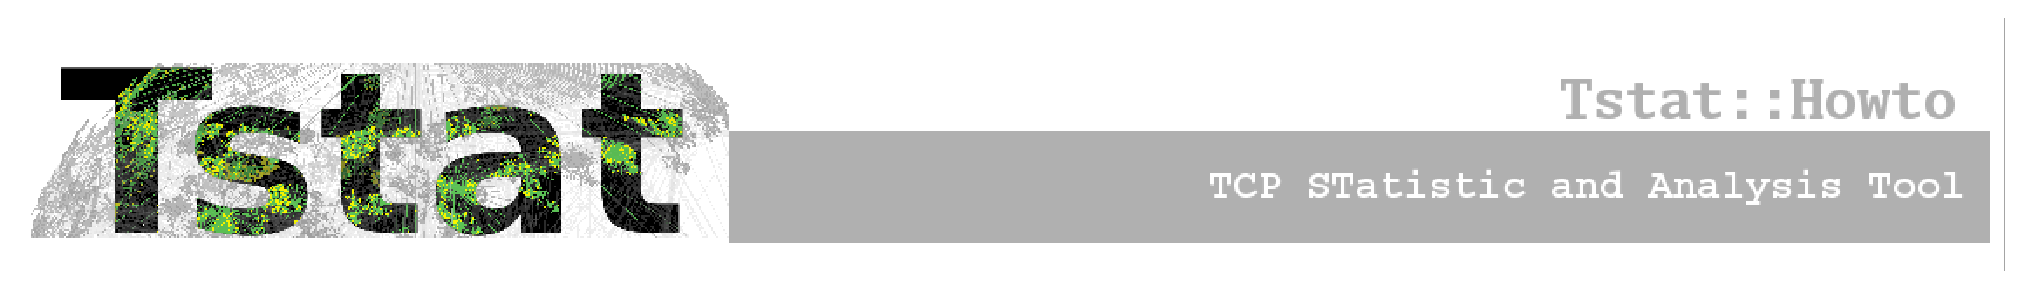
\includegraphics[width=\textwidth]{tstat_banner.eps}
    \end{center}
    \tableofcontents
    
%%  Latex generated from POD in document /home/fina/Tesi/src/tstat.autotools2-merged/doc/HOWTO-BUILD/HOWTO.pod
%%  Using the perl module Pod::LaTeX
%%  Converted on Mon Oct  6 11:03:58 2008

%%  Preamble supplied by user.

\clearpage

       %palatino
       \fontfamily{ppl}\selectfont


\section{Installation\label{Installation}\index{Installation}}


This document provides basic information
for the installation, configuration and usage 
of Tstat and the Bayesian framework for Skype
traffic identification.  A more general
description of the program as well as other
documentation can be found in the Tstat homepage
\textsf{http://tstat.tlc.polito.it}

\subsection{Requirements\label{Requirements}\index{Requirements}}
\subsubsection{Operating System\label{Operating_System}\index{Operating System}}


Tstat has been tested tested on \texttt{Linux 2.2.x}, \texttt{2.4.x} and \texttt{2.6.x} kernels, 
using \texttt{RedHat 6.x-9.x}, and \texttt{Fedora Core x} systems. 
It should work under other \texttt{UNIX} dialects, such as 
\texttt{FreeBSD}, \texttt{NetBSD 1.3} and \texttt{MAC OS X} (although we do not have any of 
those platforms for testing purposes). If you able to run Tstat on other OSs, we
will be happy to include them in the list.

\subsubsection{System Libraries\label{System_Libraries}\index{System Libraries}}


Tstat requires, by itself, a few library that should
already be installed on your system, such as 
\texttt{libpcap} (available from \textsf{http://www.tcpdump.org}) 
and the DAG drivers (available from \textsf{http://www.endace.com}), 
in case you use such hardware. With these libraries, 
you are ready to capture and process the traffic flowing
in your LAN.



Since Tstat uses pthread to improve the performance in case of real time
analysis, your system must support POSIX threads as well if you want to
profit of this feature. However, keep in mind that threaded execution 
is only an optional feature, and is necessary only for online traffic
analysis, so that this is not a strict requirement: for this reason,
threading is disabled by default.



Finally, to use the RRD functionalities, you also need to have a working
installation of RRDtool (available from \textsf{http://oss.oetiker.ch/rrdtool/}).

\subsection{Quick Install\label{Quick_Install}\index{Quick Install}}


Assuming that you want version \texttt{2.x.y}:

\begin{small}\begin{verbatim}
         wget http://tstat.polito.it/download/tstat-2.x.y.tgz
         tar -xzvf tstat-2.x.y.tgz
         cd tstat-2.x.y
         ./configure
         make
         make install (with root privileges)
\end{verbatim}\end{small} \noindent
This commands install a executable file named \texttt{tstat} in \texttt{/usr/local/bin}.

\subsection{Complete control in Build\label{Complete_control_in_Build}\index{Complete control in Build}}


The most important elements in the Tstat's package are:

\begin{small}\begin{verbatim}
    tstat/
    tstat-conf/
    libtstat/
    include/
    libtstat-demo/
    doc/ 
    doc/HOWTO
    README AUTHORS NEWS INSTALL ChangeLog
\end{verbatim}\end{small} \noindent
The \texttt{tstat} directory contains the source code of Tstat which
is also the default building target. Beside Tstat anyway, can be compiled
the \texttt{Libtstat}, a shared library which allows to an external program to access 
to the traffic analysis functions of Tstat. In the \texttt{include} directory is placed the
header file of the library instead in the \texttt{libtstat-demo} directory there is a simple 
program of example that use the Libtstat 
(see \textsf{Libtstat library} for more information about the Libtstat API).



The building of the Libtstat library is disabled by default but is provided
a configuration option to control this feature

\begin{small}\begin{verbatim}
    ./configure --enable-libtstat    # build tstat, libtstat and libtstat-demo
    ./configure                      # build only tstat
\end{verbatim}\end{small} \noindent
Tstat's source code uses some preprocess definition to enable/disable some features,
like for example the DAG support which is disabled by default.
These definitions are declared in the \texttt{tstat/Makefile.conf} each with a specific 
description about its purpose so it should be easy change to behaviour in the building
process commenting/uncommenting some lines.

\begin{description}

\item[{}] \mbox{}

NB: remember to run \texttt{autoreconf} from the root of the package every time 
a change in these file is perfomed!!!

\end{description}


The building of Libtstat is separated from the building of tstat so \texttt{libtstat/Makefile.conf}
file define the set of option specific for the Libtstat, instead \texttt{tstat/Makefile.conf}
is specific for tstat.



In the directory \texttt{tstat-conf} are placed some examples of configuration files 
needed by Tstat, for example the set of local addresses specified using -N option
or the set of protocols to dump w.r.t. the internal DPI specified with -T option.



In the directory \texttt{doc} the are some plain text files that describes the format
of logs files generated by the analysis and this howto document in different formats.
\texttt{README}, \texttt{AUTHORS}, \texttt{INSTALL}, \texttt{NEWS} and \texttt{ChangeLog} instead are plain files that
describes some general information abount the package like the authors, the last new
features of the tools ecc...

\subsection{Complete control in Install\label{Complete_control_in_Install}\index{Complete control in Install}}


The default \texttt{prefix} for installation is \texttt{/usr/local} so
Tstat executable in installed in \texttt{/usr/local/bin} and Libtstat 
is installed in \texttt{/usr/local/lib}. Anyway a different \texttt{prefix} can
be specified at configuration time

\begin{small}\begin{verbatim}
    ./configure --prefix=/absolute/path/where/install/tstat
\end{verbatim}\end{small} \noindent
Libtstat-demo is only a demostration tool so is builded only a local
executable that is not installed.



Libstat is provided with \texttt{pkg-config} support so a \texttt{libtstat.pc} is installed in
\texttt{/usr/lib/pkg-config} and typing

\begin{small}\begin{verbatim}
    pkg-config --cflags --libs libtstat
\end{verbatim}\end{small} \noindent
it should appears an output like

\begin{small}\begin{verbatim}
    -I/usr/local/include  -L/usr/local/lib -lm -lpthread -lpcap -lrrd
\end{verbatim}\end{small} \noindent
that indicates the \texttt{CFLAGS} and \texttt{LIBS} options used in the building
process.

\section{Usage\label{Usage}\index{Usage}}


There are few things to know to run Tstat: first, you are required to have a
knowledge of the network that you want to monitor. 
Second, there are the few options that are described in this section.

\subsection{Synopsis\label{Synopsis}\index{Synopsis}}


Tstat primary usage is as a command-line tool; the synopsis of 
the command is the following:

\begin{small}\begin{verbatim}
    Usage:
            tstat  [-htuvwpg] [-d[-d]] [-N file] [-s dir]
                  [-B bayes.conf] [-T dump.conf] [-S] [-L]
                  [-H ?|file ]
                  [-l] [-i interface]
                  [-f filterfile] <file1 file2>
\end{verbatim}\end{small} \noindent
\begin{small}\begin{verbatim}
    Options:
            -h: print this help and exit
            -t: print ticks showing the trace analysis progress
            -u: do not trace UDP packets
            -v: print version and exit
            -w: print [lots] of warning
            -c: concatenate the input files
                (input files should already be in the correct order)
            -p: enable multi-threaded engine (useful for live capture)
            -d: increase debug level (repeat to increase debug level)
            -N file: specify the file name which contains the
                     description of the internal networks.
                     This file must contain the subnets that will be
                     considered as 'internal' during the analysis
                     Each subnet must be specified using network IP address
                     on the first line and NETMASK on the next line:
                        130.192.0.0
                     255.255.0.0
                     193.204.134.0
                     255.255.255.0
\end{verbatim}\end{small} \noindent
\begin{small}\begin{verbatim}
            -s dir: puts the trace analysis results into directory
                   tree dir (otherwise will be <file>.out)
            -H ?: print internal histograms names and definitions
            -H file: Read histogram configuration from file
                     file describes which histograms tstat should collect
                     'include histo_name' includes a single histogram
                     'include_matching string' includes all histograms
                     whose name includes the string
                     special names are:
                     'ALL' to include all histograms
                     'ADX' to include address hits histogram
                     for example, to include all TCP related
                     and the address hits histograms, file should be:
                     include ADX
                     include_matching tcp
\end{verbatim}\end{small} \noindent
\begin{small}\begin{verbatim}
            -g: Enable global histo engine
            -S: No histo engine: do not create histograms files
            -L: No log engine: do not create log_* files
            -1: Use old (v1) log_mm format
            -B Bayes_Dir: enable Bayesian traffic classification
                      configuration files from Bayes_Dir
            -T dump.conf: configurazion file for the dump engine
            -l: enable live capture using libpcap
            -i interface: specifies the interface to be used to capture traffic
            -f fiterfile: specifies the libpcap filter file. Syntax as in tcpdump
\end{verbatim}\end{small} \noindent
\begin{small}\begin{verbatim}
            file: trace file to be analyzed
                  Use 'stdin' to read from standard input.
\end{verbatim}\end{small} \noindent
\begin{small}\begin{verbatim}
    Optional RRD options:
        -r path: path to use to create/update the RRDtool database
        -R conf: specify the configuration file for integration with 
              RRDtool. See README.RRDtool for further informetion.
\end{verbatim}\end{small} \noindent
\begin{small}\begin{verbatim}
    Optional DPMI options:
        -D conf: DPMI configuration file
\end{verbatim}\end{small} \noindent
\begin{small}\begin{verbatim}
    Note:
            When tstat is called with no arguments (on the command line),
            it will first check if a file <tstat.conf> is provided in the
            same directory where the execution started.
            In the latter case, arguments will be read from <tstat.conf>
            rather than from the command line
\end{verbatim}\end{small} \noindent
\begin{small}\begin{verbatim}
    Supported Input File Formats:
            tcpdump          tcpdump format -- Public domain program from LBL
            snoop            Sun Snoop format -- Distributed with Solaris
            etherpeek        etherpeek format -- Mac sniffer program
            netmetrix        Net Metrix format -- Commercial program from HP
            ns               ns format - Network simulator ns2 from LBL
            netscout         NetScout Manager format
            erf              Endace Extensible Record format
            DPMI             Distributed Passive Measurement Interface (DPMI) format
            tcpdump live     Live capture using pcap/tcpdump library
\end{verbatim}\end{small} \noindent
\subsection{Live Capture vs Trace Analysis\label{Live_Capture_vs_Trace_Analysis}\index{Live Capture vs Trace Analysis}}


Tstat can sniff and analyze traffic on-line through the
use of either the \texttt{libpcap} library or Endace DAG cards. 
The use of Tstat is very easy, especially if you have
experiences with \texttt{tcpdump}, although \texttt{tcpdump}'s knowledge
is not required to profitably use Tstat. Moreover, advanced 
users will enjoy the ability of on-line processing of traffic
captured with DAG cards.



As a minimal configuration, you must describe your network to Tstat. Indeed, in
order to distinguish forward and backward paths, Tstat needs  to know which host
IP addresses can be considered as ``internal'' to the monitored network. In our
case, Politecnico di Torino internal addresses are \texttt{130.192.0.0/16} and
\texttt{193.204.134.0/24}, so the network description \texttt{net.conf} looks as following:

\begin{small}\begin{verbatim}
         bash> cat net.conf
         130.192.0.0    <-- network
         255.255.0.0    <-- netmask
         193.204.134.0  
         255.255.255.0
\end{verbatim}\end{small} \noindent
We can now run Tstat to capture the traffic flowing across 
our network, with the following command, which must be run as \texttt{root} (as you
need to capture packets by putting the Ethernet interface in promiscuous mode).
The simplest command is the following:

\begin{small}\begin{verbatim}
         ./tstat -l -N net.conf
\end{verbatim}\end{small} \noindent
Beside live-capture, it is possible to run Tstat on a previously collected 
trace file, where the trace format can be any of the following:

\begin{small}\begin{verbatim}
        Supported Input File Formats:
                tcpdump          tcpdump -- Public domain program from LBL
                snoop            Sun Snoop -- Distributed with Solaris
                etherpeek        etherpeek -- Mac sniffer program
                netmetrix        Net Metrix -- Commercial program from HP
                ns               ns -- network simulator from LBL
                netscout         NetScout Manager format
                erf              Endace Extensible Record Format
                DPMI             Distributed Passive Measurement Interface (DPMI) format
                tcpdump live     Live capture using pcap/tcpdump library
\end{verbatim}\end{small} \noindent
Tstat will try to read trace files given as input, and to automatically identify
the correct dump format. Trace files can be compressed or uncompressed, and
Tstat will automatically detect the compression tool used (supported formats are
\texttt{compress, gzip, bzip2, 7z}).



Without loss of generality, we assume to use the first of the above formats. The
calling syntax is similar to the previous one, with the exception of the absence
of the live-capture switch \texttt{-l} and the presence of the name(s) of the file(s)
that have to be processed. For example, the following command can be used to
analyze a trace file named \texttt{LAN.dump.gz}. Results of the analysis
will be stored in a subdirectory named \texttt{trace1}; as before, \texttt{net.conf} contains  the
subnet description that will be considered as ``internal'' during the
analysis.

\begin{small}\begin{verbatim}
         ./tstat -s trace1 -N net.conf LAN.dump.gz
\end{verbatim}\end{small} \noindent
\subsection{More Control\label{More_Control}\index{More Control}}


We can control the interface that we want to sniff from as well as
the output directory name as follows:

\begin{small}\begin{verbatim}
         ./tstat -i eth1 -l -s test -Nnet.conf
\end{verbatim}\end{small} \noindent
Moreover, we can also pipe Tstat input using the special keyword
\texttt{stdin} as input, as in the following command (piping ns2 output to 
Tstat is left as an exercise for the reader):

\begin{small}\begin{verbatim}
         tcpdump -s 80 -i eth0 -w - ip | ./tstat -Nnet.conf -spiped stdin
\end{verbatim}\end{small} \noindent
In this case, Tstat is fed by \texttt{tcpdump}'s output, and the latter has been
instructed to capture packets on the eth0 device, collecting the
first 80 bytes (to track uniquely packet headers) of IP packets only, 
and send the output to \texttt{stdout}. Moreover, since Tstat understands 
the \texttt{libpcap} syntax, filters can be stored in text files, as in 
the following command sequence:

\begin{small}\begin{verbatim}
         echo "vlan and ip and host 10.0.0.1" > tcpdump.conf
         ./tstat  -i eth0 -l -f tcpdump.conf -N net.conf -s filtered
\end{verbatim}\end{small} \noindent
\section{Output\label{Output}\index{Output}}
\subsection{Output Classification\label{Output_Classification}\index{Output Classification}}


Recall that Tstat assumes that traces are collected on a bidirectional link,
such that both data and control packets belonging to the same flow are observed;
with the help of the figures below, we will explain the different classification
of measurements used by Tstat.



         \begin{figure}[!htb]
             \begin{center}
                 \includegraphics[width=0.6\textwidth]{tstat_output.eps}
             \end{center}
         \end{figure}





Tstat identifies hosts based on their IP address. Given the description
of the internal hosts through the \texttt{-N} command line option, Tstat
distinguishes among \textit{incoming}, \textit{outgoing} and \textit{local} 
measurements. Packets whose destination is an internal host and whose source is
an external host will contribute to \textit{incoming} measurements (red arrow in the
top figure), whereas packets going
in the opposite direction will contribute to \textit{outgoing} measurements (green
arrow in the top figure). Finally, in
some cases it is possible that Tstat observes packets whose source and
destination host belong to the internal host set: in such cases, measurements
will be classified as \textit{local} (blue arrow in the top figure).
Notice that packets whose source and destination IP
addresses belong to the external host set will be discarded.
For example, consider a setup in which Tstat is attached to a snoop port of a
LAN switch. Then Tstat will be fed by i) \textit{outgoing} packets going to the default gateway,
ii) \textit{incoming} packets coming from the default gateway, iii) \textit{local} packets.



Note that if you either do not know or do not want to distinguish between
internal, external and local hosts, you may enable the \texttt{-DLOG\_UNKNOWN}
directive when compiling Tstat. Tstat will then be less strict, but results may
be difficult to be correctly interpreted.



Considering instead the \textit{role} of the host that sent the packet, statistic are
collected distinguishing between \textit{clients} (green arrow in the bottom figure)
and \textit{servers} (red arrow in the top figure), i.e., host
that opens a connection and and host that replies to connection request. Recall
that while TCP connections are well defined, UDP (and RTP/RTCP) connection
definition is more fuzzy. In this latter case, Tstat will consider as client the
source IP address of the host that sent the first packet of that flow, while the
server will be the host identified by the destination IP address of the same
packet.



Therefore, when applicable, Tstat will keep track of measurements referring to
the same measured quantity by \textit{appending} a specific tag  to the filename:

\begin{description}

\item[{\texttt{\_out}}] \mbox{}

outgoing: from an internal host to an external host


\item[{\texttt{\_in}}] \mbox{}

incoming: from an external host to an internal host


\item[{\texttt{\_loc}}] \mbox{}

local between two internal hosts


\item[{\texttt{\_c2s}}] \mbox{}

going from the Client to the Server


\item[{\texttt{\_s2c}}] \mbox{}

going from the Server to the Client

\end{description}
\subsection{Output Structure\label{Output_Structure}\index{Output Structure}}


Tstat collects several network-layer as well as transport-layer measurements,
which are described in full details in \textsf{http://tstat.polito.it/measure.shtml}.
As output, Tstat produces three different types of measurement collections, which
will be described in the current section:

\begin{description}

\item[{Histograms}] \mbox{}

store the \textit{distribution} of a given quantity within a time interval.


\item[{Round Robin Database}] \mbox{}

stores a configurable subset of the same quantities through the RRD interface.


\item[{Log files}] \mbox{}

store a complete transport-layer \textit{log} of all the parameters measured.

\end{description}
\subsection{Output Types\label{Output_Types}\index{Output Types}}


This section details the different \textit{types} of measurement collections
generated by Tstat; for detailed informations on  the specific \textit{metrics} 
that Tstat is able to gather, please refer to the Tstat website 
\textsf{http://tstat.polito.it/measure.shtml}.

\subsubsection{Histograms\label{Histograms}\index{Histograms}}


Histograms are generated periodically: Tstat collects all the
measurement data during a given measurement interval defined by the \texttt{MAX\_TIME\_STEP} 
parameter, which is hard-coded in the \texttt{param.h} file to 5 minutes. Please, note
that changing the \texttt{MAX\_TIME\_STEP} parameter may affect RRD creation as well.
For example, considering the IP packet length, Tstat updates, for
each observed IP packet, the counter of the number of observed packets with a
particular length. At the end of the measurement period, Tstat then saves
the values stored in the histogram, resets all the values, and then restarts 
the samples collection.



Considering the last example of previous section, we run:

\begin{small}\begin{verbatim}
         ./tstat -s trace1 -N net.conf 23_00_28_Jun_2000.dump.gz
\end{verbatim}\end{small} \noindent
The output generated by tstat consists of a directory tree like the following:

\begin{small}\begin{verbatim}
        trace1
        `-- 23_00_28_Jun_2000.out
            |-- 000
            |   |-- addresses
            |   |-- flow_number
            |   |-- ip_len_in
            |   ...
            |   |-- udp_port_flow_dst
            |   `-- udp_tot_time
            |-- 001
            |   |-- addresses
            |   |-- flow_number
            |   |-- ip_len_in
            |   ...
            |   |-- udp_port_flow_dst
            |   `-- udp_tot_time
            ...
            |-- LAST
            |   |-- addresses
            |   |-- flow_number
            |   |-- ip_len_in
            |   ...
            |   |-- udp_port_flow_dst
            |   `-- udp_tot_time
            |-- log_rtp_complete
            |-- log_tcp_complete
            `-- log_tcp_nocomplete
\end{verbatim}\end{small} \noindent
\begin{itemize}

\item Main database

The topmost directory is created according to the command line option \texttt{-s},
which in this case is set to \texttt{trace1}. This is intended to be the main database
directory.


\item Trace Start Time

A subdirectory named from the timestamp of the first tracked packet is created using
the \texttt{"\%H\_\%M\_\%d\_\%b\_\%Y.out"} (or, in a more  human readable format,
\texttt{hour\_minute\_day\_Month\_year.out/}) notation. When running in live mode (c$<$-l$>$
option), a new directory with the name of the current tracked packet Timestamp
will be created every \texttt{DIRS*MAX\_TIME\_STEP} time. The parameter \texttt{DIRS} is
defined in the file \texttt{param.h} as well. By default it is set to 12, so that a
new dir will be approximatively created every hour of live measurement.


\item Collection Interval

Subdirectories with increasing numbers will be created for each measurement
period with the format \texttt{nnn/}; histograms collecting measurement results will
be created in these directories; note that the histograms referring to the last
\textit{partial} time period will be stored in the LAST subdirectory. The option \texttt{-g}
adds also the subdirectory GLOBAL containing the gloabl histogrmas for the whole
measurement period.


\item Histogram data

Each of these \texttt{nnn/}  directories contain several histograms, one for each of 
the measured parameters, relative to the nnn-th \texttt{MAX\_TIME\_STEP} long time interval;
notice that the tags \texttt{\_in}, \texttt{\_out}, \texttt{\_loc}, \texttt{\_c2s} and \texttt{\_s2c}
are appended to indicate the classification of the observed stream.



Histogram data are saved using simple ASCII files.
The format is simple: the first line contains a description of the
measured quantity, while the second line contains the parameters of the histograms
(minimum and maximum values, and size of each bins). The list of all
the counter index and values is then dumped. To limit the file size, the
corresponding entry is omitted if the counter is zero.
For example, the histogram of the packet length \texttt{ip\_len\_in} looks like:

\begin{small}\begin{verbatim}
     #IP packet length - incoming packets
     #min=0 bin_size=4 max=1600
     28 7
     36 277
     40 11760
     44 3463
     ...
\end{verbatim}\end{small} \noindent
\end{itemize}


Simple \textsf{Post Processing} tools are available to automatically manage the histogram
database.

\subsubsection{RRD\label{RRD}\index{RRD}}


The RRD output consists of a series of binary files stored in the RRD format.
Tstat forces a particular \textit{naming notation} of such files, which follows
the configuration rules described later in Sec.~\ref{RRD_Configuration}.



The RRD can then be queried with the standard RRDtool commands, such as
\texttt{rrdcreate}, \texttt{ rrdupdate},  \texttt{ rrdgraph}, \texttt{ rrddump}, \texttt{ rrdfetch}, 
\texttt{ rrdtune}, \texttt{ rrdlast}, \texttt{ rrdxport}, to whose manual pages we refer 
the reader for further informations.

\subsubsection{Logs\label{Logs}\index{Logs}}


Tstat creates three transport-layer log-files: \texttt{log\_tcp\_complete},
\texttt{log\_tcp\_nocomplete} and \texttt{log\_rtp\_complete}. 
Log files are placed in the main database directory.



TCP flows can be either completed or not depending whether Tstat observed the
3-way handshaking or not; in the first case, all the measured indexes relatively
to each flow will be collected in the \texttt{log\_tcp\_complete}; in the latter
case,  flows are considered as garbage and stored in \texttt{log\_tcp\_nocomplete};



Similarly, a complete log keeping track of each UDP flow measured indexes is
maintained in the \texttt{log\_udp\_complete} file. Being UDP basically a
connectionless protocol, it is impossible to distinguish among \texttt{complete} and
\texttt{nocomplete} flows in this case.



Furthermore the following log filesa are created: \texttt{log\_mm\_complete} for multimedia flows
(i.e. RTP, RTCP, etc), \texttt{log\_chat\_complete} for chating protocols (i.e. MSN, jabber, etc) and
\texttt{log\_skype\_complete} for skype traffic.



Description of the file format of the log files can be found in
\textsf{http://tstat.polito.it/measure.shtml}.

\subsubsection{Traces\label{Traces}\index{Traces}}


Tstat internally has a \texttt{Deep Packet Inspector - DPI} which is able to identify
traffic communications at application level looking the composition of the payload
of packets. Using the \texttt{-T} command line option, specifing a configuration file,
is possibile to split the input traffic (readed from a trace or from an network card)
in traces with the respect to the classification operated by the DPI.



The syntax of the dump configuration file is really simple:

\begin{small}\begin{verbatim}
    > cat tstat-2.x.y/tstat-conf/dump.conf
    [udp]           # indicate the set of UDP protocols
    rtp
    rtcp
    edk
    kad
    kadu
    gnutella
    bittorrent
    dc
    kazaa
    pplive
    sopcast
    tvants
    unknown         # all the traffic that the DPI don't recognize
    complete        # all the traffic
\end{verbatim}\end{small} \noindent
The previous list indicate the complete list of protocols of which it can be generated
a trace, and, as it can be seen, this feature is for now available only for UDP
traffic. In the \texttt{tstat-conf} directory of the package there is complete example of
this file that can be modified commenting/uncommenting lines to enable/disable
the tracking of specific protocols.



The traces generated are placed in a subdirectory 
named \texttt{traces} inside the output directory and the traffic
is splitted in traces with windows of 1 hour. This means that, for example,
if we start the dump at 9:00 am

\begin{small}\begin{verbatim}
    traces/complete.pcap0       #traffic from 9:00  to 10:00
    traces/complete.pcap1       #traffic from 10:00 to 11:00
    ...
\end{verbatim}\end{small} \noindent
\subsection{Post Processing\label{Post_Processing}\index{Post Processing}}


This section could be a separate HOWTO, since this
argument cannot be treated exhaustively. Perl, Awk, Ruby
\textit{Your-Favorite-Scripting-Language} scripts are definitively
best candidates to post-process \texttt{log\_*} files.



In the Tstat download page, you
can find \texttt{plot\_time.pl} and \texttt{plot\_cum.pl}, two Perl scripts that may be useful
to produce either i) time or ii) aggregated plots over different time spans.
They directly access the histogram database created by Tstat.
Please, refer to \textsf{http://tstat.polito.it/software.php\#postprocess}.



RRD files can be manipulated to obtain \textit{indirect} 
metrics through the RPN manipulations mechanism provided 
by RRDtool.

\subsection{Storage Considerations\label{Storage_Considerations}\index{Storage Considerations}}


To give the user a rough idea of the size of the output,
let us consider a 6 hours long, 1.6GB packet-level trace containing 
21M packets, sniffed with \texttt{tcpdump} that was used throughout this tutorial.
Tstat identified and analyzed about 729K flows, of which about 495K were 
TCP flows, trashing 20K of them into \texttt{log\_nocomplete}.
Referring to the Sec.~\ref{Output_Structure} above shown,
we can express the following observations:

\begin{description}

\item[{Histogram}] \mbox{}

As previously described, in order to take into account the flow directions,
several histograms are dumped for the same variable \texttt{var\_\{in,out,loc,c2s,s2c\}}.
Currently, about 60 measurement indexes, described in 
\textsf{http://tstat.tlc.polito.it/measure.shtml},  are logged, for a total
of 180 files. Each of the \texttt{000/}, \texttt{001/} ... \texttt{LAST/} directories is about
500KB-1MB depending on the network traffic and on the file system block
allocation mechanism.



Therefore,  as a rule of thumb, you can count about 1MB of storage due to
histograms every 5 minutes of traffic (independently of the amount of actual
traffic load during the 5 mins...). This can be useful in order to set the
periodic dump timer to the desired trade off among time granularity versus
storage size  required.


\item[{RRD}] \mbox{}

The \texttt{rrd/} directory is, per construction, of fixed size: this should not be a
surprise, since this is the goal of RRD. Therefore, the size of the database
does not depend on the amount of network traffic processed, but rather on the
RRD configuration. For the standard configuration supplied with Tstat, which is
also the one used in our Web server, the whole database occupy only 6MB and
consists of about 250 files.


\item[{Logs}] \mbox{}

The total size of the log files amount to about 200MB, which 
gives  a 8x reduction factor w.r.t. the packet-level trace; or,
the storage cost of each flow is about 400 bytes.



Note that the \texttt{log\_*} can be further compressed, using \texttt{gzip}
to less than 50MB, which gives a further 4x size gain; 
however, for a matter of performance, is preferable 
to compress the log files \textit{offline}.

\end{description}


Finally, consider that on a common PC architecture (specifically,
Intel P4 2.40GHz equipped with 2GB of RAM and 7200rpm hard-disk),
the whole trace elaboration took only 4 minutes; thus, the 
analysis rate is roughly 85Kpkts/sec or 3Kflows/sec.

\section{RRD Module\label{RRD_Module}\index{RRD Module}}
\subsection{RRDtool Installation\label{RRDtool_Installation}\index{RRDtool Installation}}


In order to get Tstat RRD module working, you will need to install RRDtool first
(refer to the homepage of RRDtool \textsf{http://oss.oetiker.ch/rrdtool/}  to accomplish this step).
Then, make sure to specify that you want native RRD support in Tstat by
modifying the \texttt{Makefile} accordingly, and (re)compile Tstat: you will have to
uncomment the following lines in \texttt{Makefile}, and  to double-check
that the RRDtool version and path are coherent with your system settings.

\begin{small}\begin{verbatim}
   DEFINES    += -DHAVE_RRDTOOL
   RRD_VER     = 1.2.9
   RRD_LDLIBS  = -lrrd
   RRD_LDFLAGS = -L/usr/lib/ -L/usr/rrdtool/lib/  -L/usr/rrdtool-${RRD_VER}/lib/
   RRD_INCS    = -I/usr/rrdtool/include/ -I/usr/rrdtool-${RRD_VER}/include
\end{verbatim}\end{small} \noindent
If someone is willing to integrate the RRD identification and configuration
directly via the \texttt{configure}, we would appreciate it!

\subsection{RRD Configuration\label{RRD_Configuration}\index{RRD Configuration}}


Tstat RRD configuration is very easy, being centralized
in a single text-file, which allows to specify at runtime what measurements
should be monitored. The operating frequencies
for the RRD sampling (i.e., the parameters for the temporal 
averages) are hard-coded into \texttt{rrdtool.h} and are chosen to 
mimic MRTG behavior. Again, take care that modifying the \texttt{MAX\_TIME\_STEP}
parameter may affect the RRD management as well.



The RRD configuration file, specified through the command line option \texttt{-R},
should contain one line for each of the Tstat parameters that have
to be integrated into a Round Robin Database. Each line allows to
specify which statistical properties of the variable has to be tracked,
as follows:

\begin{small}\begin{verbatim}
          tstat_var1 avg min max stdev var val:a,b,c,d idx:e,f,g,h,other prc:i,j,k
\end{verbatim}\end{small} \noindent
where \texttt{avg,min,max,stdev,var,idx,prc,other} are keywords, whereas \texttt{a,b,c,d,i,j,k} 
are floating point numbers and \texttt{e,f,g,h} integer values; note that
the list of indexes (e.g., TCP ports), values (e.g., packet size)
and percentiles are comma separated. The name of the variables are
Tstat internal ones: they can be seen by executing \texttt{./tstat -H},
Alternatively, you can directly look into the \texttt{000/} ...  \texttt{LAST/}  directories or
or at \textsf{http://tstat.polito.it/measure.shtml}



Valid configuration lines are, e.g.:

\begin{small}\begin{verbatim}
          #
          # inspect IP packet length average, specific values and distribution
          #
          ip_len_in   avg prc:50,90,95,99 idx:40,1500,other
\end{verbatim}\end{small} \noindent
\begin{small}\begin{verbatim}
          #
          # TCP well known ports       
          #                       
          # 20    FTP-DATA             
          # 21    FTP                  
          # 22    SSH                  
          # 23    telnet               
          # 25    SMTP                 
          # 80    HTTP                 
          # ...                        
          #
          tcp_port_dst_in       idx:20,21,22,23,25,80,other
\end{verbatim}\end{small} \noindent
\begin{small}\begin{verbatim}
          #
          # good approximation of the distribution of the RTT,
          # taking into account only the incoming path contribution
          #
          tcp_rtt_avg_in  prc:0.1,1,5,10,25,50,75,90,95,99,99.9
\end{verbatim}\end{small} \noindent
where, evidently, the lines starting with a \texttt{\#} sign are treated as comments.
Our Web server is currently running with the configuration
available at \textsf{http://tstat.polito.it/download/rrd.conf}.



For each specified quantity defined in the rrd.conf file, a corresponding file
will be created.
For example, consider that the generic configuration line:

\begin{small}\begin{verbatim}
          tstat_var avg min max stdev var val:a,b,c,d idx:e,f,g,h,other prc:i,j,k
\end{verbatim}\end{small} \noindent
will produce the following files (17 in total):

\begin{small}\begin{verbatim}
          tstat_var.{avg,min,max,stdev,var}.rrd
          tstat_var.val{a,b,c,d}.rrd
          tstat_var.idx{e,f,g,h,oth}.rrd
          tstat_var.prc{i,j,k}.rrd
\end{verbatim}\end{small} \noindent
\subsection{Tstat RRD and the Web\label{Tstat_RRD_and_the_Web}\index{Tstat RRD and the Web}}


From the Tstat web site, you can
download the most up-to-date version of \texttt{tstat\_rrd.cgi},
which is the CGI script that renders the Web interface.
Here is some basic tips to get it working; if you wonder
how to write your own graph templates, then you are probably
skilled enough to get it on your own \texttt{:)}

\subsubsection{Database Structure\label{Database_Structure}\index{Database Structure}}


The CGI scripts allow to browse on the fly the RRD database structure.
The \texttt{rrd\_data} directory is the root of the tree, where each
directory contains either i) other directories (i.e., is a box) 
or ii) a RRD-database, in which case the node is a leaf and will be
shown in the interface. In case that a directory is a plain box, it may
optionally contain some files (specifically 
\{\texttt{HEADER},\texttt{FOOTER},\texttt{README}\}.\{\texttt{html},\texttt{txt}\})
that will be rendered by \texttt{tstat\_rrd.cgi}. 
By default, the cgi script tries to load the html version;
otherwise, it tries to displays "$<$pre$>$ `cat FILE` $<$/pre$>$"
if such a FILE exists; finally, it will display a default message
held in \$default\{README\} hard coded in the script.



Here is an example of the rrd\_data directory which holds part of the RDD database
accessible from the tstat web page.

\begin{small}\begin{verbatim}
        rrd_data/
         |-- Example
         |-- GARR
         |   |-- garr-live
         |   `-- garr-old
         `-- Polito
             |-- 2000
             |   |-- Apr
             |   |-- Jun
             |   |-- Jun,post155
             |   `-- May
             |-- 2001
             |   |-- Feb
             |   `-- Jan
             |-- 2005
             |   |-- Apr
             |   `-- Feb
             `-- Current
\end{verbatim}\end{small} \noindent
\subsubsection{Web Configuration\label{Web_Configuration}\index{Web Configuration}}


The web configuration really depends on your web server configuration. Few
dependencies are required, most notably, the RRD Perl library from the RRDtool
installation.



It is advisable to store the Tstat RRD files
everywhere you want, and then create a symbolic link 
named \texttt{rrd\_data} that points to it (i.e., to the root of 
the rrd database tree). Similarly for the directory
where the rendered images should be stored (defaults to \texttt{cgi-bin/rrd\_images})
and can be a symbolic link as well.
The names of these symbolic links can be redefined in the 
configuration section of \texttt{tstat\_rrd.cgi} if needed:

\begin{small}\begin{verbatim}
        #   ____________________________
        #  /                            \
        # /    configuration  __________/
        # \__________________/.:nonsns:.
        #
        # specify path to the root of the rrd database tree
        # by default, I assume there is a symbolic link in cgi-bin/
        # named rrd_data
        $RRD_DATA = 'rrd_data';
\end{verbatim}\end{small} \noindent
\begin{small}\begin{verbatim}
        # same thing for image directory
        # in my case, var/www/cgi-bin/rrd_images is
        # a symbolic link to "/var/www/html/rrd_images";
        # from the html browser's perspective
        $IMG_DIR = "rrd_images";
\end{verbatim}\end{small} \noindent
\section{DPMI Module\label{DPMI_Module}\index{DPMI Module}}


To the experienced DPMI user, it can turn very useful to
think of Tstat in terms of a DPMI consumer, thus suitable
for live usage. Basically, two configuration files need to 
be provided in this case.

\subsection{Tstat Configuration for DPMI\label{Tstat_Configuration_for_DPMI}\index{Tstat Configuration for DPMI}}


Especially for this purpose,  Tstat can be executed without any argument
on the command line, provided that a file named \texttt{tstat.conf} 
exists in the same path where the \texttt{tstat} command has been
executed. Note that the filename MUST be in this case \texttt{tstat.conf}



In the latter case, arguments will be read from 
\texttt{tstat.conf} rather than from the command line, which makes
Web-based execution easier -- it just requires the creation of
a text file.



Typically, the content of the file will be one of the two following
cases. When only the RRD module need to be turned on, which is 
specially suitable for the persistent monitoring of a network link:

\begin{small}\begin{verbatim}
          -D dpmi.conf -S -R rrd.conf -r data.rrd
\end{verbatim}\end{small} \noindent
Or, in the case where more detailed transport layer logs and histograms 
are to be generated, such as for shorter ad-hoc experiment:

\begin{small}\begin{verbatim}
          -D dpmi.conf -s data
\end{verbatim}\end{small} \noindent
Note that the \texttt{dpmi.conf} filename, which is the object of the next 
section, is customizable.

\subsection{DPMI Configuration for Tstat\label{DPMI_Configuration_for_Tstat}\index{DPMI Configuration for Tstat}}


This file is used by Tstat in order to properly set-up the 
DPMI library and, possibly, its filters. There are only two
keywords that are interpreted by Tstat, and \textit{the whole} 
content of this file is passed to the DPMI's \texttt{createfiler}
library call.
Tstat-keywords are prepended by the \texttt{tstat:} prefix, to 
solve any ambiguity, and are related to the type of stream
and measurement direction.
More specifically,

\begin{description}

\item[{\texttt{tstat:(file$|$(tcp$|$udp$|$eth)[:port])}}] \mbox{}

Specify whether a tracefile or a network socket (and in this case, which port)
is the source of DPMI traffic. Note that in the case where a tracefile
is used, there is no real need to specify this, since the format recognition
happens automatically; thus, the \texttt{tstat:file} keyword is provided for completeness.
Conversely, options such as \texttt{tstat:eth} and \texttt{tstat:tcp:32449} are
necessary in order for network sokets to properly be setup.


\item[{\texttt{tstat:MP:CI}}] \mbox{}

This option is used to define the traffic directionality, specifing 
what network card interface (CI) and the measurement point (MP) 
are related to \textit{incoming} traffic from external sources.
Referring to the DPMI library internals:

\begin{small}\begin{verbatim}
      CI <-> char nic[8];     
      MP <-> char mampid[8];
\end{verbatim}\end{small} \noindent
\end{description}


In order to provide a safe failback or a missing configuration,
unless otherwise specified, the first received frame is assumed to 
be ``incoming'', thus arbitrarily determinining the incoming CI:MP 
couple.

\section{Bayesian Classification of Skype Traffic\label{Bayesian_Classification_of_Skype_Traffic}\index{Bayesian Classification of Skype Traffic}}


This section deals with the task of configuring and tuning the 
Bayesian framework integrated within Tstat.

\subsection{A Simple Example\label{A_Simple_Example}\index{A Simple Example}}


Assuming that you have configured the Bayesian classifier (a proper configuration sample 
for the Bayesian detection of Skype traffic is provided in the \texttt{skype} directory), 
traffic identification can be carried on either on-line or off-line: in both cases, 
a per-flow logfile will be created as output.

\begin{small}\begin{verbatim}
        ./tstat -l -B skype -N net.conf
\end{verbatim}\end{small} \noindent
\begin{small}\begin{verbatim}
        ./tstat -B skype -N net.conf tracefile.dump
\end{verbatim}\end{small} \noindent
\subsection{Framework Configuration\label{Framework_Configuration}\index{Framework Configuration}}


The Bayesian framework is configured through a directory name, 
containing several configuration files. A default configuration
is provided under the \texttt{tstat-conf} directory: 
there are two main files that allow to finely tune the framework, 
as described in details below.
These files specify the parameter settings for different 
Naive Bayes Classifiers (NBC), corresponding to different features 
of the flows. As features, the framework consider 
the \textbf{packet size} (\texttt{pktsize.conf}) and \textbf{average inter-packet gap}
(\texttt{avgipg.conf}).



Each of these files has the format specified in the example below, where lines 
starting with a dash sign \texttt{\#} are interpreted as comments.

\begin{small}\begin{verbatim}
           #   ____________________________  
           #  /                            \ 
           # /    BayesConf      __________/ 
           # \__________________/.:nonsns:.  
           #                              
           #===============================================
           # feature name
           #-----------------------------------------------
           # Known Skype features:
           #    PKTSIZE 
           #    MAXDELPKTSIZE  
           #    AVGIPG  
           #    PKTRATE  
           #    BITRATE  
           #
           FEATURE      AVGIPG
           #
           #===============================================
           # default flags 
           #-----------------------------------------------
           # USE_LOG        1
           # NORMALIZE      1
           # AUTO_OTHER     0
           #
           WINDOW_SIZE      1
           CLASS_LEN        250
           MIN_THRESHOLD    1e-25
           AVG_THRESHOLD   -3.5
           WIN_THRESHOLD   -3
           #
           #===============================================
           # class definition
           #-----------------------------------------------
           # syntax
           #    DISCRETE  class P{class}
           #    GAUSSIAN  class P{class} mu sigma
           #    GAUSSIAN+ class P{class} N (w1,m1,s1) .. (wN,mN,sN)
           #
           # note: P{class} may be "="
           #
           GAUSSIAN mode1 = 10 2
           GAUSSIAN mode2 = 20 2
           GAUSSIAN mode3 = 30 2
           GAUSSIAN mode4 = 40 2
           GAUSSIAN mode5 = 50 2
           GAUSSIAN mode6 = 60 2
\end{verbatim}\end{small} \noindent
First of all, the feature name is defined, then some optional parameters are set
(such as the window size, the optional use of logarithms to avoid underflows in 
Bayesian belief computation, the use of normalization, etc.).



Minimum threshold avoids underflows in Bayesian belief computation,
the max mean belief is compared against the average threshold to decide
whether the flow can be considered skype or non-skype and the window
threshold is used to count the number of individual samples (rather than
their mean) that passes a more restrictive test (indeed the window threshold
is greater than the average threshold).



Finally, different classes for the given feature are defined, which correspond to different
``modes''. Such classes may be represented as gaussian (or superposition of gaussian) distributions,
centered over a given mean and with a  given standard deviation, or may be arbitrarily specified (discrete 
distribution). The class probability is equally shared among the classes by the keyword 
\texttt{=} as in the example above. As we will see, changing the order of the class definition
affects the meaning of some of the logfile fields values.

\section{Libtstat library\label{Libtstat_library}\index{Libtstat library}}


As described in the Install section of this document, to enable the building of
Libtstat library is needed to provide a configure option

\begin{small}\begin{verbatim}
    ./configure --enable-libtstat
\end{verbatim}\end{small} \noindent
\subsection{Link the Libtstat library\label{Link_the_Libtstat_library}\index{Link the Libtstat library}}


When the library is installed in the system using \texttt{make install} the
following messages are printed on the console

\begin{small}\begin{verbatim}
    ----------------------------------------------------------------------
    Libraries have been installed in:
    /usr/local/lib
\end{verbatim}\end{small} \noindent
\begin{small}\begin{verbatim}
    If you ever happen to want to link against installed libraries
    in a given directory, LIBDIR, you must either use libtool, and
    specify the full pathname of the library, or use the `-LLIBDIR'
    flag during linking and do at least one of the following:
    - add LIBDIR to the `LD_LIBRARY_PATH' environment variable
      during execution
    - add LIBDIR to the `LD_RUN_PATH' environment variable
      during linking
    - use the `-Wl,--rpath -Wl,LIBDIR' linker flag
    - have your system administrator add LIBDIR to `/etc/ld.so.conf'
\end{verbatim}\end{small} \noindent
\begin{small}\begin{verbatim}
    See any operating system documentation about shared libraries for
    more information, such as the ld(1) and ld.so(8) manual pages.
    ----------------------------------------------------------------------
\end{verbatim}\end{small} \noindent
This indicate where the library has been installed and how to
link that to some program. The most simple thing to do, is to 
use the native libtool support for automake, that is, assuming
that \texttt{program\_name} is the name of the executable of the tool
to generate, it is needed to add the following lines to \texttt{Makefile.am}
of the tool:

\begin{small}\begin{verbatim}
    program_name_LDADD = -ltstat -lpcap -lpthread -lm
    program_name_LDFLAGS = -Wl,--rpath -Wl,<libtstat_dir>
\end{verbatim}\end{small} \noindent
This allow a fined control on the directory where the library 
has been installed. Anyway, if it has been installed in a
standard library location (as \texttt{/usr/lib}), instead of the previous
lines, it can be added

\begin{small}\begin{verbatim}
    AC_CHECK_LIB([tstat], [tstat_next_pckt],, AC_MSG_ERROR([missing 'tstat' library]))
\end{verbatim}\end{small} \noindent
in \texttt{configure.ac} of the current project. This automatically
look for the presence of a function tstat\_next\_pckt() in a system library
named \texttt{libtstat}. In case of error of error print a message stopping the
configuration process, instead in case of success, are automatically added
all the linking options needed to build the program (see the autotools 
files in \texttt{libtstat-demo} for a complete example).

\subsection{Libtstat API\label{Libtstat_API}\index{Libtstat API}}
\begin{description}

\item[{int tstat\_init (char *config\_fname)}] \mbox{}

\texttt{config\_fname} is a file name containing a set of Tstat options, one 
for each line

\begin{small}\begin{verbatim}
    >cat tstat-conf/tstat.conf
    #-s outdir      # output directory
    -N net.all      # network config file 
    #-B bayesdir    # directory of the bayes config files
    #-d             # debug
\end{verbatim}\end{small} \noindent
If NULL is provided, the library use \texttt{./tstat.conf} as filename.


\item[{void tstat\_new\_logdir (char *filename,}] \textbf{struct timeval *pckt\_time)}

This function has to be called before the process of the first packet
and allow to generate the output directory using this hierarchy:

\begin{small}\begin{verbatim}
    <filename>.out
        |__<pckt_time>.out
\end{verbatim}\end{small} \noindent
\item[{int tstat\_next\_pckt (struct timeval *pckt\_time,}] \textbf{void *ip\_hdr, void *last\_ip\_byte, int tlen)}

This function enable the processing of a new packet.
\texttt{pckt\_time}  is the timestamp of the packet, \texttt{ip\_hdr} is a pointer to the first ip byte,
\texttt{last\_ip\_byte} is a pointer to the last ip byte, and \texttt{tlen} is the number of total bytes (captured).


\item[{tstat\_report *tstat\_close (tstat\_report}] \textbf{*report)}

This function flush to file all the pending statistics
and fill a tstat\_report structure with some general
results.


\item[{void tstat\_print\_report (tstat\_report}] \textbf{*report, FILE *file)}

This function print a formatted report to file
using tstat\_report data.

\end{description}
\section{Author Informations\label{Author_Informations}\index{Author Informations}}
\begin{small}\begin{verbatim}
        Marco Mellia, Assistant Professor.
        <marco.mellia@polito.it>
\end{verbatim}\end{small} \noindent
\begin{small}\begin{verbatim}
        Dario Rossi, PostDoc Researcher.
        <dario.rossi@polito.it>
\end{verbatim}\end{small} \noindent
\begin{small}\begin{verbatim}
        Dario Bonfiglio, Researcher.
        <bonfiglio@serverlipar.polito.it>
\end{verbatim}\end{small} \noindent
\begin{small}\begin{verbatim}
        Telecommunication Networks Group (TNG)
        DELEN, Politecnico di Torino
        http://www.tlc-networks.polito.it
\end{verbatim}\end{small} \noindent
\section{Acknowledgment\label{Acknowledgment}\index{Acknowledgment}}


Many people contributed to the development of Tstat. Tstat would never have seen
the light had not \texttt{TCPTrace} being invented.
Many thanks to Shawn Ostermann and to the  Ohio
University for their great program.



Many Master and PhD students took part in the development and debugging of
Tstat. Naming all of them would be impossible. We would then like to thank Luca
Muscariello for the entropy generated in the TCP
anomalies identification, and Prof. Marco Ajmone Marsan and 
Prof. Fabio Neri who gave us the moral and scientific support to 
continue investing in Tstat.

\section{License\label{License}\index{License}}


Copyright (c) 2001 Politecnico di Torino.  All rights reserved.



This program is free software; you can redistribute it and/or modify
it under the terms of the GNU General Public License as published by
the Free Software Foundation; either version 2 of the License, or
(at your option) any later version.

\printindex

\end{document}
